\chapter{graph objects}
\label{graphobj} \index{graph object} \index{visualizing data}

{\em Author: Andreas Brezger} \\
\vspace{0.3cm}


{\em Graph objects} are used to visualize data and estimation
results obtained by other objects in {\em BayesX}. Currently {\em
graph objects} can be used to draw scatterplots between variables
(\autoref{graphplot} method #plot#), or to draw and color
geographical maps stored in {\em map objects}
(\autoref{graphdrawmap} method #drawmap#). The obtained plots are
either printed on the screen or stored as a postscript file for
further use in other documents (e.g. \LaTeX\/ documents).
A {\em graph object} is created by typing

#> graph# {\em objectname}

in the {\em command window}.



\clearpage



\section{Method drawmap}
\label{graphdrawmap} \index{graph object!drawmap command}
\index{drawing geographical maps}

\begin{stanza}{Description}

{Method #drawmap# is used to draw geographical maps and color the
regions according to some numerical characteristics.}
\end{stanza}

\begin{stanza}{Syntax}

 #> #{\em objectname}.#drawmap#  [{\em plotvar regionvar}] [#if# {\em expression}], {\em #map#=mapname} [{\em options}]
 [#using# {\em dataset}]

Method #drawmap# draws the map stored in the {\em map object} {\em
mapname} and prints the graph either on the screen or stores it as
a postscript file (if option #outfile# is specified). The regions
with regioncode {\em regionvar} are colored according to the
values of the variable {\em plotvar}. The variables {\em plotvar}
and {\em regionvar} are supposed to be stored in the {\em dataset
object} {\em dataset}. An #if# statement may be specified to use
only a part of the data in {\em dataset}. Several options are
available, e.g. for changing from grey scale to color scale or
storing the map as a postscript file. See the options list below
for more details.
\end{stanza}

\begin{stanza}{Options}

{The most important option, which must always be specified, is the
#map# option. Here the name of the {\em map object} containing the
boundary information of the map to be drawn is specified. The
following options are available for method #drawmap# (in
alphabetical order):}
\end{stanza}

\begin{itemize}
\item #color#

The #color# option allows to choose between a grey scale for the
colors and a colored scale. If #color# is specified a colored
scale is used instead of a grey scale.

\item #drawnames#

In some situations it may be useful to print the names of the
regions into the graph (although the result may be confusing in
most cases). This can be done by specifying the additional option
#drawnames#. By default the names of the regions are omitted in
the map.

\item #fontsize = #{\em integer}

Specifies the font size (in pixels) for labelling the legend and
writing the names of the regions (if specified). Note, that the
title is scaled accordingly (see option #titlesize#). The default is
#fontsize=12#.

\item #hcl#

Requests that a color palette from the HCL color space should be
used instead of an RGB palette. The HCL colors will be selected
diverging from a neutral center (grey) to two different extreme
colors (red and green) in contrast to the RGB colors diverging from
yellow to red and green. HCL colors are particularly useful for
electronic presentations since they are device-independent. The
option #hcl# is only meaningful in combination with the option
#color#.

\item #lowerlimit = #{\em realvalue}

Lower limit of the range to be drawn. If #lowerlimit# is omitted,
the minimum numerical value in {\em plotvar} will be used as the
lower limit instead.

\item #map = #{\em mapname}

{\em mapname} specifies the name of the {\em map object}
containing the boundary information of the map to be drawn. This
option must always be specified.

\item #nolegend#

By default a legend is drawn into the graph. By specifying the
option #nolegend# the legend will be omitted.

\item #nrcolors = #{\em integer}

To color the regions according to their numerical characteristics,
the data are divided into a (typically large) number of ordered
categories. Afterwards a color is associated with each category.
The #nrcolors# option can be used to specify the number of
categories (and with it the number of different colors). The
maximum number of colors is 256, which is also the default value.

\item #outfile = #{\em filename}

If option #outfile# is specified the graph will be stored as a
postscript file rather than being printed on the screen. The path
and the filename must be specified in {\em filename}. By
default, an error will be raised if the specified file  is already
existing or the specified folder is not existing. To overwrite  an
already existing file, option #replace# must be additionally
specified. This prevents you from unintentionally overwriting your
files.

\item #pcat#

If you want to visualize posterior probabilities it is convenient to
specify #pcat#. This forces #drawmap# to expect a column that
consists only of the values -1, 0 and 1. Of course you can achieve
the same result by setting #nrcolors=3#, #lowerlimit=-1# and
#upperlimit=1#.

\item #replace#

The #replace# option is only useful in combination with option
#outfile#. Specifying #replace# as an additional option allows the
program to overwrite an already existing file (specified in
#outfile#), otherwise an error will be raised.

\item #swapcolors#

In some situations it may be favorable to swap the order of the
colors, i.e. black (red) shades corresponding to large values and
white (green) shades corresponding to small values. This is
achieved by specifying #swapcolors#. By default, small values are
colored in black shades (red shades) and large values in white
shades (green shades).

\item #title = #{\em characterstring}

Adds a title to the graph. If the title contains more than one
word, {\em characterstring} must be enclosed by quotation marks
(e.g. #title="my first map"#).

\item #titlesize = #{\em realvalue}

Specifies the factor by which the size of the title is scaled
relative to the size of the labels of the legend (compare option
#fontsize#). The default is \texttt{titlesize=1.5}.

\item #upperlimit = #{\em realvalue}

Upper limit of the range to be drawn. If #upperlimit# is omitted,
the maximum numerical value in {\em plotvar} will be used as the
upper limit instead.

\end{itemize}

\begin{stanza}{Example}

This example shows how to draw the map of Munich and how to color
the subquarters in Munich according to some numerical
characteristics. You find the boundary file of Munich (#munich.bnd#)
as well as the data set #rent94means.raw# containing the
distribution of the average rents across subquarters in the
subfolder #examples# of your {\em BayesX} installation directory. In
the following we assume that {\em BayesX} is installed in the folder
#c:\bayesx#. We first create a {\em dataset object} #d# and a {\em
map object} #m# and read in the rent data set and the map of Munich:

#> dataset d# \\
#> d.infile using c:\bayesx\examples\rent94means.raw#

#> map m# \\
#> m.infile using c:\bayesx\examples\munich.bnd#

We proceed by creating a {\em graph object} #g# and by drawing the map of Munich:

#> graph g# \\
#> g.drawmap , map=m#

\begin{figure}[htb]
\begin{center}
\includegraphics[scale=0.5]{grafiken/munichdrawmap.ps}
{\em\caption{ \label{munichdrawmap} Map of Munich}}
\end{center}
\end{figure}

The map of Munich appears on the screen in a separate window, see
\autoref{munichdrawmap}. Before closing the window you are asked
whether you want to save the map or not. If you agree the map will
be stored as a postscript file in the folder you specify. Of
course, the map can be directly stored in postscript format using
the #outfile# option. In that case the map is not shown on the
screen. Typing

#> g.drawmap , map=m outfile=c:\temp\munich.ps#

stores the map of Munich in the file
#c:\temp\munich.ps# and the graph is not
being printed on the screen.

Usually maps are drawn to visualize numerical characteristics of
their regions. For instance,
by typing

#> g.drawmap R L , map=m color using d#

the distribution of the average rents #R# across subquarters #L# are
displayed, see \autoref{munichmeans}. The areas in the figure shaded
with diagonal lines mark subquarters for which  no data are
available. The specification of the second variable #L# is required
to match the names of the subquarters stored in the {\em map object}
#m# with the data set #d#. Option #color# is specified to obtain a
colored graph. Specifying option #hcl# in addition yields the same
information visualized in HCL colors (see \autoref{munichmeanshcl}).

#> g.drawmap R L , map=m color hcl using d#

\end{stanza}

\begin{figure}[htb]
\begin{center}
\includegraphics[scale=0.5]{grafiken/munichmeansdrawmap.ps}
{\em\caption{ \label{munichmeans} Distribution of the average rents
per square meter in Munich visualized in RGB colors.}}
\end{center}
\end{figure}

\begin{figure}[htb]
\begin{center}
\includegraphics[scale=0.5]{grafiken/munichmeansdrawmaphcl.ps}
{\em\caption{ \label{munichmeanshcl} Distribution of the average
rents per square meter in Munich visualized in HCL colors.}}
\end{center}
\end{figure}

\clearpage



\section{Method plot}
\label{graphplot} \index{graph object!plot command}
\index{scatterplot} \index{drawing scatterplots}

\begin{stanza}{Description}

{Method #plot# is used to draw scatterplots between two or more
variables. Several options for labelling axes, connecting points,
saving the graph etc. are available.}
\end{stanza}

\begin{stanza}{Syntax}

{#> #{\em objectname}.#plot#  {\em xvar yvar1} [{\em yvar2 yvar3}
\dots]
[#if# {\em expression}] [, {\em options}] #using# {\em dataset}

Method #plot# draws scatterplots of {\em yvar1}, {\em yvar2}, {\em
yvar3} $\dots$ against {\em xvar} into a single graph using the
data set specified in {\em dataset}. An #if# statement may be used
to apply the method only to a part of the data. In addition,
several options may be specified for labelling axes, connecting
points, saving the graph in postscript format etc., see the
options list below.}
\end{stanza}

\begin{stanza}{Options}

{The following options are available for method #plot# (listed in
alphabetical order):}
\end{stanza}

\begin{itemize}
\item #connect = 1#$|$#2#$|$#3#$|$#4#$|$#5#[{\em specifications
for further variables}]

Option #connect# specifies how points in the scatterplot are
connected. There are currently 5 different specifications:

\begin{tabular}{ll}
#1# & draw straight lines between the points (default) \\
#2#, #3#, #4# & draw dashed lines (numbers 2-4 indicate different variants)\\
#5# & do not connect, i.e.~plot points only \\
\end{tabular}

If you draw more than one scatterplot in the same graph (i.e. more
than one {\em yvar} is specified) you can connect points for every
{\em yvar} differently by simply specifying the corresponding number
(#1,2,3,4,5#) for every {\em yvar}. Typing for example

#connect=15#

connects the points corresponding to {\em yvar1} and {\em xvar} by
straight lines, but does not connect the points corresponding to
{\em yvar2} (if specified) and {\em xvar}. Points corresponding to
additionally specified variables $yvar3$, etc.~are connected by
straight lines.

An equivalent way of specifying the different variants is
available via the symbols '#l#', '#d#', '#_#', '#-#' and '#p#',
which correspond to the numbers 1-5, i.e.~

#connect=12345# is equivalent to #connect=ld_-p#

\item #fontsize = #{\em integer}

Specifies the font size (in pixels) for labelling axes etc. Note
that the title is scaled accordingly. The default is
#fontsize=12#.

\item #height = #{\em integer}

Specifies the height (in pixels) of the graph. The default is
#height=210#.

 \item #linecolor = B#$|$#b#$|$#c#$|$#G#$|$#g#$|$#o#$|$#m#$|$#r#$|$#y# [{\em specifications
for further variables}]

Option #linecolor# specifies the color to be used for drawing
lines (or points, see option #connect#) in the scatterplot.
Currently the following specifications are available:

\begin{tabular}{ll}
#B# & black (default) \\
#b# & blue \\
#c# & cyan \\
#G# & gray \\
#g# & green \\
#o# & orange \\
#m# & magenta \\
#r# & red \\
#y# & yellow \\
\end{tabular}

If you draw more than one scatterplot in the same graph (i.e. more
than one {\em yvar} is specified) you can use different colors for
each {\em yvar} by simply specifying the corresponding symbol
(#B,b,c,G,g,o,m,r,y#) for each {\em yvar}. Typing for example

#linecolor = Bgr#

colors the lines (points) corresponding to {\em yvar1} and {\em
xvar} in black, whereas the points corresponding to {\em yvar2}
and {\em yvar3} (if specified) and {\em xvar} are colored in green
and red, respectively.

\item #linewidth = #{\em integer}

Specifies how thick lines should be drawn. The default is
#linewidth=5#.

\item #outfile = #{\em filename}

If option #outfile# is specified the graph will be stored as a
postscript file rather than being printed on the screen. The path
and the filename must be specified in {\em filename}. By default,
an error will be raised if the specified file is already existing
or the specified folder is not existing. To overwrite  an already
existing file, option #replace# must be additionally specified.
This prevents you from unintentionally overwriting your files.

\item #pointsize = #{\em integer}

Specifies the size of the points (in pixels) if drawing points
rather than lines is specified. The default is #pointsize=20#.

\item #replace#

The #replace# option is useful only in combination with option
#outfile#. Specifying #replace# as an additional option allows the
program to overwrite an already existing file (specified in
#outfile#), otherwise an error will be raised.

\item #title = #{\em characterstring}

Adds a title to the graph. If the title contains more than one
word, {\em characterstring} must be enclosed by quotation marks (e.g.
#title="my first title"#).

\item #titlesize = #{\em realvalue}

Specifies the factor by which the size of the title is scaled
relative to the size of the labels of the axes (compare option
#fontsize#). The default is \texttt{titlesize=1.5}.

\item #width = #{\em integer}

Specifies the width (in pixels) of the graph. The default is
#width=356#.

\item #xlab = #{\em characterstring}

Labels the x-axis. If the label contains more than one word, {\em
characterstring} must be enclosed by quotation marks (e.g.
#xlab="x axis"#).

\item #xlimbottom = #{\em realvalue}

Specifies the minimum value at the x-axis to be drawn. The default
is the minimum value in the data set. If #xlimbottom# is above the
minimum value in the data set, only a part of the  graph will be
visible.

\item #xlimtop = #{\em realvalue}

Specifies the maximum value at the x-axis to be drawn. The default
is the maximum value in the data set. If #xlimtop# is below the
maximum value in the data set, only a part of the  graph will be
visible.

\item #xstart = #{\em realvalue}

Specifies the value where the first 'tick' on the x-axis should be
drawn. The default is the minimum value on the x-axis.

\item #xstep = #{\em realvalue}

If #xstep# is specified,  ticks are drawn at the x-axis with
stepwidth {\em realvalue} starting at the minimum value on the
x-axis (or at the value specified in option #xstart#). By default,
five equally spaced ticks are drawn at the x-axis.

\item #ylab = #{\em characterstring}

Labels the y-axis. If the label contains more than one word, {\em
characterstring} must be enclosed by quotation marks (e.g.
\texttt{ylab="y axis"}).

\item #ylimbottom = #{\em realvalue}

Specifies the minimum value at the y-axis to be drawn. The default
is the minimum value in the data set. If #ylimbottom# is above the
minimum value in the data set, only a part of the  graph will be
visible.

\item #ylimtop = #{\em realvalue}

Specifies the maximum value at the y-axis to be drawn. The default
is the maximum value in the data set. If #ylimtop# is below the
maximum value in the data set, only a part of the  graph will be
visible.

\item #ystart = #{\em realvalue}

Specifies the value where the first 'tick' on the y-axis should be
drawn. The default is the minimum value on the y-axis.

\item #ystep = #{\em realvalue}

If #ystep# is specified,  ticks are drawn at the y-axis with
stepwidth {\em realvalue} starting at the minimum value on the
y-axis (or at the value specified in option #ystart#). By default,
five equally spaced ticks are drawn at the y-axis.

\item Further options

In the following we describe options that may be useful if the
variable at the x-axis represents dates. An example is a variable
with values ranging from 1 to 19 representing the time period from
January 1983 to July 1984. In this case, we naturally prefer that
the x-axis is labelled in terms of dates rather than in the
original coding (form 1 to 19). To achieve this we provide the
options #month#, #year# and #xstep#. Options #year# and #month#
are used to specify the year and the month (1 for January, 2 for
February, \dots) corresponding to the minimum covariate value. In
the example mentioned above #year=1983# and #month=1# will produce
the correct result. In addition, option #xstep# may be specified
to define the periodicity in which your data are collected. For
example #xstep=12# (the default) corresponds to monthly data,
while #xstep = 4#, #xstep = 2# and #xstep = 1# correspond to
quarterly, half yearly and yearly data.
\end{itemize}


\begin{stanza}{Example}

{We use the Munich rent data set #rent94.raw# to demonstrate the
usage of method #plot#. You find the data set #rent94.raw# in the
subfolder #examples# of your {\em BayesX} installation directory.
In the following we assume that {\em BayesX} is installed in the
folder #c:\bayesx#.
We first read in the data by typing:

#> dataset d# \\
#> d.infile using c:\bayesx\examples\rent94.raw#

We now generate a {\em graph object} #g# and draw a scatterplot
between floor space (variable #F#)
and rent per square meter (variable #R#):

#> graph g# \\
#> g.plot R F using d#

The strange picture shown in \autoref{plotrf1} appears on the
screen. The problem is that the points are connected by straight
lines and that the values of #F# are not sorted. Hence, to obtain
an improved scatterplot we could either sort the data set with
respect to #F# or simply avoid connecting the points.
Typing

#> d.sort F# \\
#> g.plot R F using d#

yields the first option. Typing

#> g.plot R F , connect=p using d#

yields the second option mentioned above. The corresponding graphs
are shown in \autoref{plotrf2} and \autoref{plotrf3},
respectively. To further improve the appearance of the scatterplot
we add a title and label the x- and y-axes
by typing

#> g.plot R F , title="scatterplot between F and R" ylab="rent"# \\
#  xlab="floor space in square meters" connect=p using d#

The result is shown in \autoref{plotrf4}.
Finally, we add the outfile option to save the graph in postscript format:

 #> g.plot R F , title="scatterplot between F and R" ylab="rent" #\\
 #  xlab="floor space in square meters" connect=p#\\
 #  outfile=c:\temp\plotrf.ps using d #

\begin{figure}[ht]
\begin{center}
\includegraphics[scale=0.7]{grafiken/plotrf1.ps}
{\em\caption{ \label{plotrf1} Scatterplot between floor space and
rent per square meters (first try).}}
\end{center}
\end{figure}

\begin{figure}[ht]
\begin{center}
\includegraphics[scale=0.7]{grafiken/plotrf2.ps}
{\em\caption{ \label{plotrf2} Scatterplot between floor space and
rent per square meters (second try).}}
\end{center}
\end{figure}

\begin{figure}[ht]
\begin{center}
\includegraphics[scale=0.7]{grafiken/plotrf3.ps}
{\em\caption{ \label{plotrf3} Scatterplot between floor space and
rent per square meters (third try).}}
\end{center}
\end{figure}

\begin{figure}[ht]
\begin{center}
\includegraphics[scale=0.7]{grafiken/plotrf4.ps}
{\em\caption{ \label{plotrf4} Scatterplot between floor space and
rent per square meters (final try).}}
\end{center}
\end{figure}
}
\end{stanza}
\clearpage



\clearpage



\section{Method plotautocor}
\label{graphplotautocor} \index{graph object!plotautocor command}
\index{plotting autocorrelations}

\begin{stanza}{Description}

{Method #plotautocor# visualizes the autocorrelation functions
obtained with method #autocor# of {\em bayesreg objects}, see also
\autoref{bayesautocorr}.}
\end{stanza}


\begin{stanza}{Syntax}

{#> #{\em objectname}.#plotautocor# [,{\em options}] #using# {\em dataset}

Plots the autocorrelation functions stored in {\em dataset}. The
data set must have the special structure described in
\autoref{bayesautocorr}, i.e. method #plotautocor# is meaningful
only if Bayesian regression models have been estimated in advance
using {\em bayesreg objects} and autocorrelation functions of
sampled parameters have been computed using method #autocor# of
{\em bayesreg objects}.}
\end{stanza}

\subheader{Options}

\begin{itemize}
\item #mean#

If option #mean# is specified, for each lag number and model term
only minimum, mean and maximum autocorrelations are plotted. This
can lead to a considerable reduction in computing time and storing
size.

\item #outfile = #{\em filename}

If option #outfile# is specified the graph will be stored as a
postscript file and not printed on the screen. The path and the
filename must be specified in {\em filename}. An error will be
raised if the specified file is already existing and the #replace#
option is not specified.

\item #replace#

The #replace# option is only useful in combination with option
#outfile#. Specifying #replace# as an additional option allows the
program to overwrite an already existing file (specified in
#outfile#), otherwise an error will be raised.
\end{itemize}



\clearpage



\section{Method plotsample}
\label{graphplotsample} \index{graph object!plotsample command}
\index{plotting sampled parameters} \index{sampling paths}

\begin{stanza}{Description}

{Method #plotsample# visualizes the sampling paths of sampled
parameters obtained with method #getsample# of {\em bayesreg
objects}, see also \autoref{bayesgetsample}. The application of
method #plotsample# is meaningful only if Bayesian regression
models have been estimated in advance using {\em bayesreg objects}
and sampled parameters have been computed and stored using method
#getsample# of {\em bayesreg objects}.}
\end{stanza}

\begin{stanza}{Syntax}

{#> #{\em objectname}.#plotsample# [,{\em options}] #using# {\em dataset}

Plots sampled parameters stored in {\em dataset}. The data set
must have the special structure described in
\autoref{bayesgetsample}.}
\end{stanza}

\subheader{Options}

\begin{itemize}
\item #outfile = #{\em filename}

If option #outfile# is specified the graph will be stored as a
postscript file and not printed on the screen. The path and the
filename must be specified in {\em filename}. An error will be
raised if the specified file is already existing and the #replace#
option is not specified (see below).

\item #replace#

The #replace# option is only useful in combination with option
#outfile#. Specifying #replace# as an additional option allows the
program to overwrite an already existing file (specified in
#outfile#), otherwise an error will be raised.
\end{itemize}
